\documentclass{article}
\usepackage[utf8]{inputenc}
\title{Video 3:The Mathematics Behind Principal Component Analysis }
\author{wbg231 }
\date{December 2022}
\newcommand{\R}{$\mathbb{R}$}
\newcommand{\B}{$\beta$}
\newcommand{\A}{$\alpha$}
\newcommand{\D}{\Delta}

\newcommand{\avector}[2]{(#1_2,\ldots,#1_{#2})}
\newcommand{\makedef}[2]{$\textbf{#1}$:#2 }
\usepackage{tikz,graphicx,hyperref,amsmath,amsfonts,amscd,amssymb,bm,cite,epsfig,epsf,url}

\begin{document}

\maketitle

\section*{introduction}
\begin{itemize}
\item \href{https://www.youtube.com/watch?v=l9qIW_UBiZs}{vedio link}
\item today we are talking about the math behind pca
\subsection*{pca}
\item we are going to focus on PCA of a dataset (but we showed that the same thing holds for a random vector)
\item the steps of pca for a given dataset $X$ are 
\begin{enumerate}
    \item compute sample covariance matrix $\Sigma_{X}$
    \item do the eigen decomposition of $\Sigma_{X}$ to get Principal directions $u_1...u_d$
    \item center the data and compute Components directions by projecting our data onto each Principal direction that is $w_j[i]=u_{j}^{t}ct(x_i), \quad \forall i\in [1,n], j\in [1,d]$
    \item where $ct(x_i)=x_i-M(x)$
\end{enumerate}
\item this allows us to find the directions of maximal variance, as well as the Components of our data that capture the maximal variance
\item he then goes through an example, which we did in last Video so i am not going to write it down again 
\subsection*{maximizing variance}
\item so recall given a dataset we can find the variance of our dataset in a 
 in a certain direction $b\in \mathbb{R}^{d}$ as the variance of our dataset projected
 onto that direction a
\item so our dataset X projected onto direction a is $X_{a}=\{a^tx_1...x^tx_n\}$
\item and thus the variance of our dataset in that direction is given by $var(X_a)=a^t\Sigma_{X}a$ 
which we can call $q(a)$
\item we can look at this function over the set $A=\{a\in \mathbb{R}^{d}:||a||=1\}$ that is $q(A)$
\item which when graphed looks like this along the contour lines of some dataset  \\ \includegraphics*[width=4cm]{notes/week_8/Vedio_3/immages/v3_1.png}
\item then we can look at the values $Q(A)$ it's self in  \\ \includegraphics*[width=4cm]{notes/week_8/Vedio_3/immages/v3_2.png}
\item so how can we maximize this function representing variance in every direction?
\subsection*{will there be a max}
\item first we want to show there must be a maximal value for this function
\item first off we know $q(a)=a^t\Sigma_{X}a$ is continuous 
\item  and we know the set we are looking at (A) the unit sphere is closed and bounded thus there must be a max by the extreme value theorem
\item t
\subsection*{what will this max look like?}
\item to look at the max of $q(a)=a^t\Sigma_{X}a$ we want to reason about it's gradient 
\item we know that $\Sigma_{X}$ is symmetric thus $\nabla_{a}q(a)=2\Sigma_{X}a$
\item that looks like this\\ 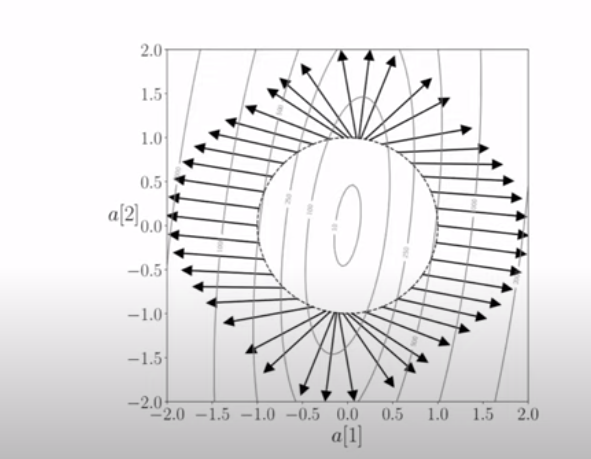
\includegraphics[width=4cm]{notes/week_8/Vedio_3/immages/v3_3.png}
\item the gradient encodes the directional derivative of $q(a)$
\item the directional derivative of $q(a)$ in the direction of some unit vector b is given by 
$q'(b)=lim_{\epsilon\rightarrow 0}\frac{q(b+\epsilon h)-q(b)}{\epsilon}=(\nabla q(b))^th$ so it is the gradient of the quadratic form and h 
\item so in other words $q'(b)>0 \Rightarrow q(b+\epsilon h)>q(b)$ for some $\epsilon>0$
\item  at the max $u_1$ we can not have $(\nabla q(u_1))^{t}h\geq 0$ for any $u_1+\epsilon h$ in the constrained set (So in this case on the unit sphere)
\item so we can not stay on the constrained set if we move in the constrained set 
\subsection*{tangent hyperplane}
\item the unit sphere is a level surface of the function $s(a):a^ta$
\item so the unit sphere is the set given by $A:=\{a:s(a)=1\}$
\item we know a vector $y\in \mathbb{R}^{d}$ is in the tangent plane of $A$ at be if $$\nabla s(a)^{t}(y-b)=0$$ that is saying that the vector y-b must be orthogonal to our gradient at b 
\item this is important because we are in this case because as we are moving we are almost staying at the same value of $s(a)$ in this case on the unit circle
\item so we can then write if y-b is small ie y and b are close $$s(y)\approx s(b)+\nabla(y-b)^{t}$$
\item that is we are almost staying on the circle
\item so graphically we have \\ \includegraphics*[width=4cm]{notes/week_8/Vedio_3/immages/v3_4.png}
\subsection*{maximizing q }
\item so given what we showed above when can a point maximize q(a)
\item \begin{itemize}
\item so for h such that $b+\epsilon h$ is on our tangent plane and we have $$\nabla(b)^{T}g=q'(b)>0\Rightarrow q(b+\epsilon h)>q(b)$$
\item for some b in the tangent plane, then we can use a taylor approximation to find a a $y\approx (b+\epsilon h)$ where $y$ is on the unit cricle
\item this means we can move within our constrained set (ie within the circle) and increase our function value (so that point can not be a max of q(a))
\end{itemize}
\item so when will  a point be a max of $q(a)$ there should be no $h$ such that $b+\epsilon h$ is in our level set an $\nabla(b)^th=q'(b)> 0$
\item so in other words we need the gradient of our level set to be orthogonal to our hyperplane and thus colinear with the gradient of $s(b)$
\item so in our case the gradient of $q(s)$ $\nabla q(s)$ must be orthogonal to the circle to achieve a max \\ \includegraphics*[width=4cm]{notes/week_8/Vedio_3/immages/v3_5.png}
\item this is equivlent to having a point $u_1$ such that $\nabla q(u_1)\parallel \nabla s(u_1)$ ie $q'(u_1)=0$
\item so this tells us at the max/min of $q(a)$ there must be some scaler $\lambda$ such that $\nabla q(u)=\lambda s(u)\iff  q(u)\parallel \nabla s(u)$
\item we know that $g(a)=a^t\Sigma_{X}a$ and thus $\nabla q(u)=2\Sigma_{X} u$
\item and that $s(a)=a^ta$ and thus $\nabla s(u)=2u$ 
\item so we want  $2\Sigma_{x}u=2\lambda u\Rightarrow \Sigma_{x}u=\lambda u$ in other words u must be an eigenvector of $\Sigma x$ 
\item and clearly that is maximized at the largest eigenvector $u_1$ corresponding to the largest eigenvalue $\lambda_1$
\item this establishes the spectral theorem, which we used in the lsat Video
\end{itemize}
\end{document}
